\section{Méthodologie}

La méthodologie suivie dans le cadre de ce projet repose sur une approche structurée et progressive, visant à garantir une migration des données précise et adaptée aux besoins spécifiques du client. 

\subsection{Localisation des informations sur l’ancien logiciel du client}

La première étape du projet consiste à localiser les informations nécessaires dans l’ancien logiciel utilisé par le client. Cette phase est cruciale, car elle permet d’identifier précisément où et comment sont structurées les données client qu'il serait intéressant de reprendre. 
On a donc un accès temporaire au précédent logiciel du client pour nous permettre de réaliser cette tâche. Dans le cas du SSTI03, le précédent se nomme préventiel.

\begin{figure}[h!]
  \centering
  % Première image
  \begin{subfigure}{0.35\textwidth} % Largeur relative à la page
      \centering
      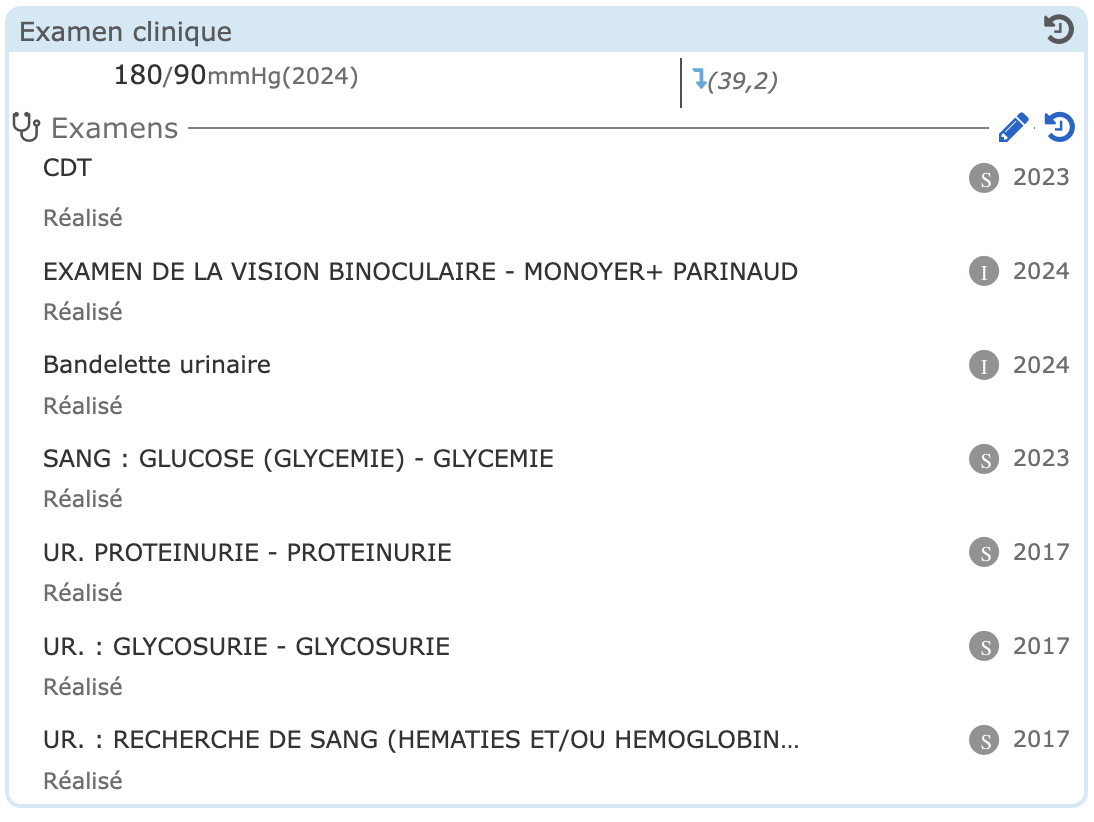
\includegraphics[width=\linewidth]{4_attachments/figures/preventiel_exam.png} % Remplacez "image1.png"
      \caption{Aperçu}
      \label{fig:image1}
  \end{subfigure}
  \hfill
  % Deuxième image
  \begin{subfigure}{0.55\textwidth}
      \centering
      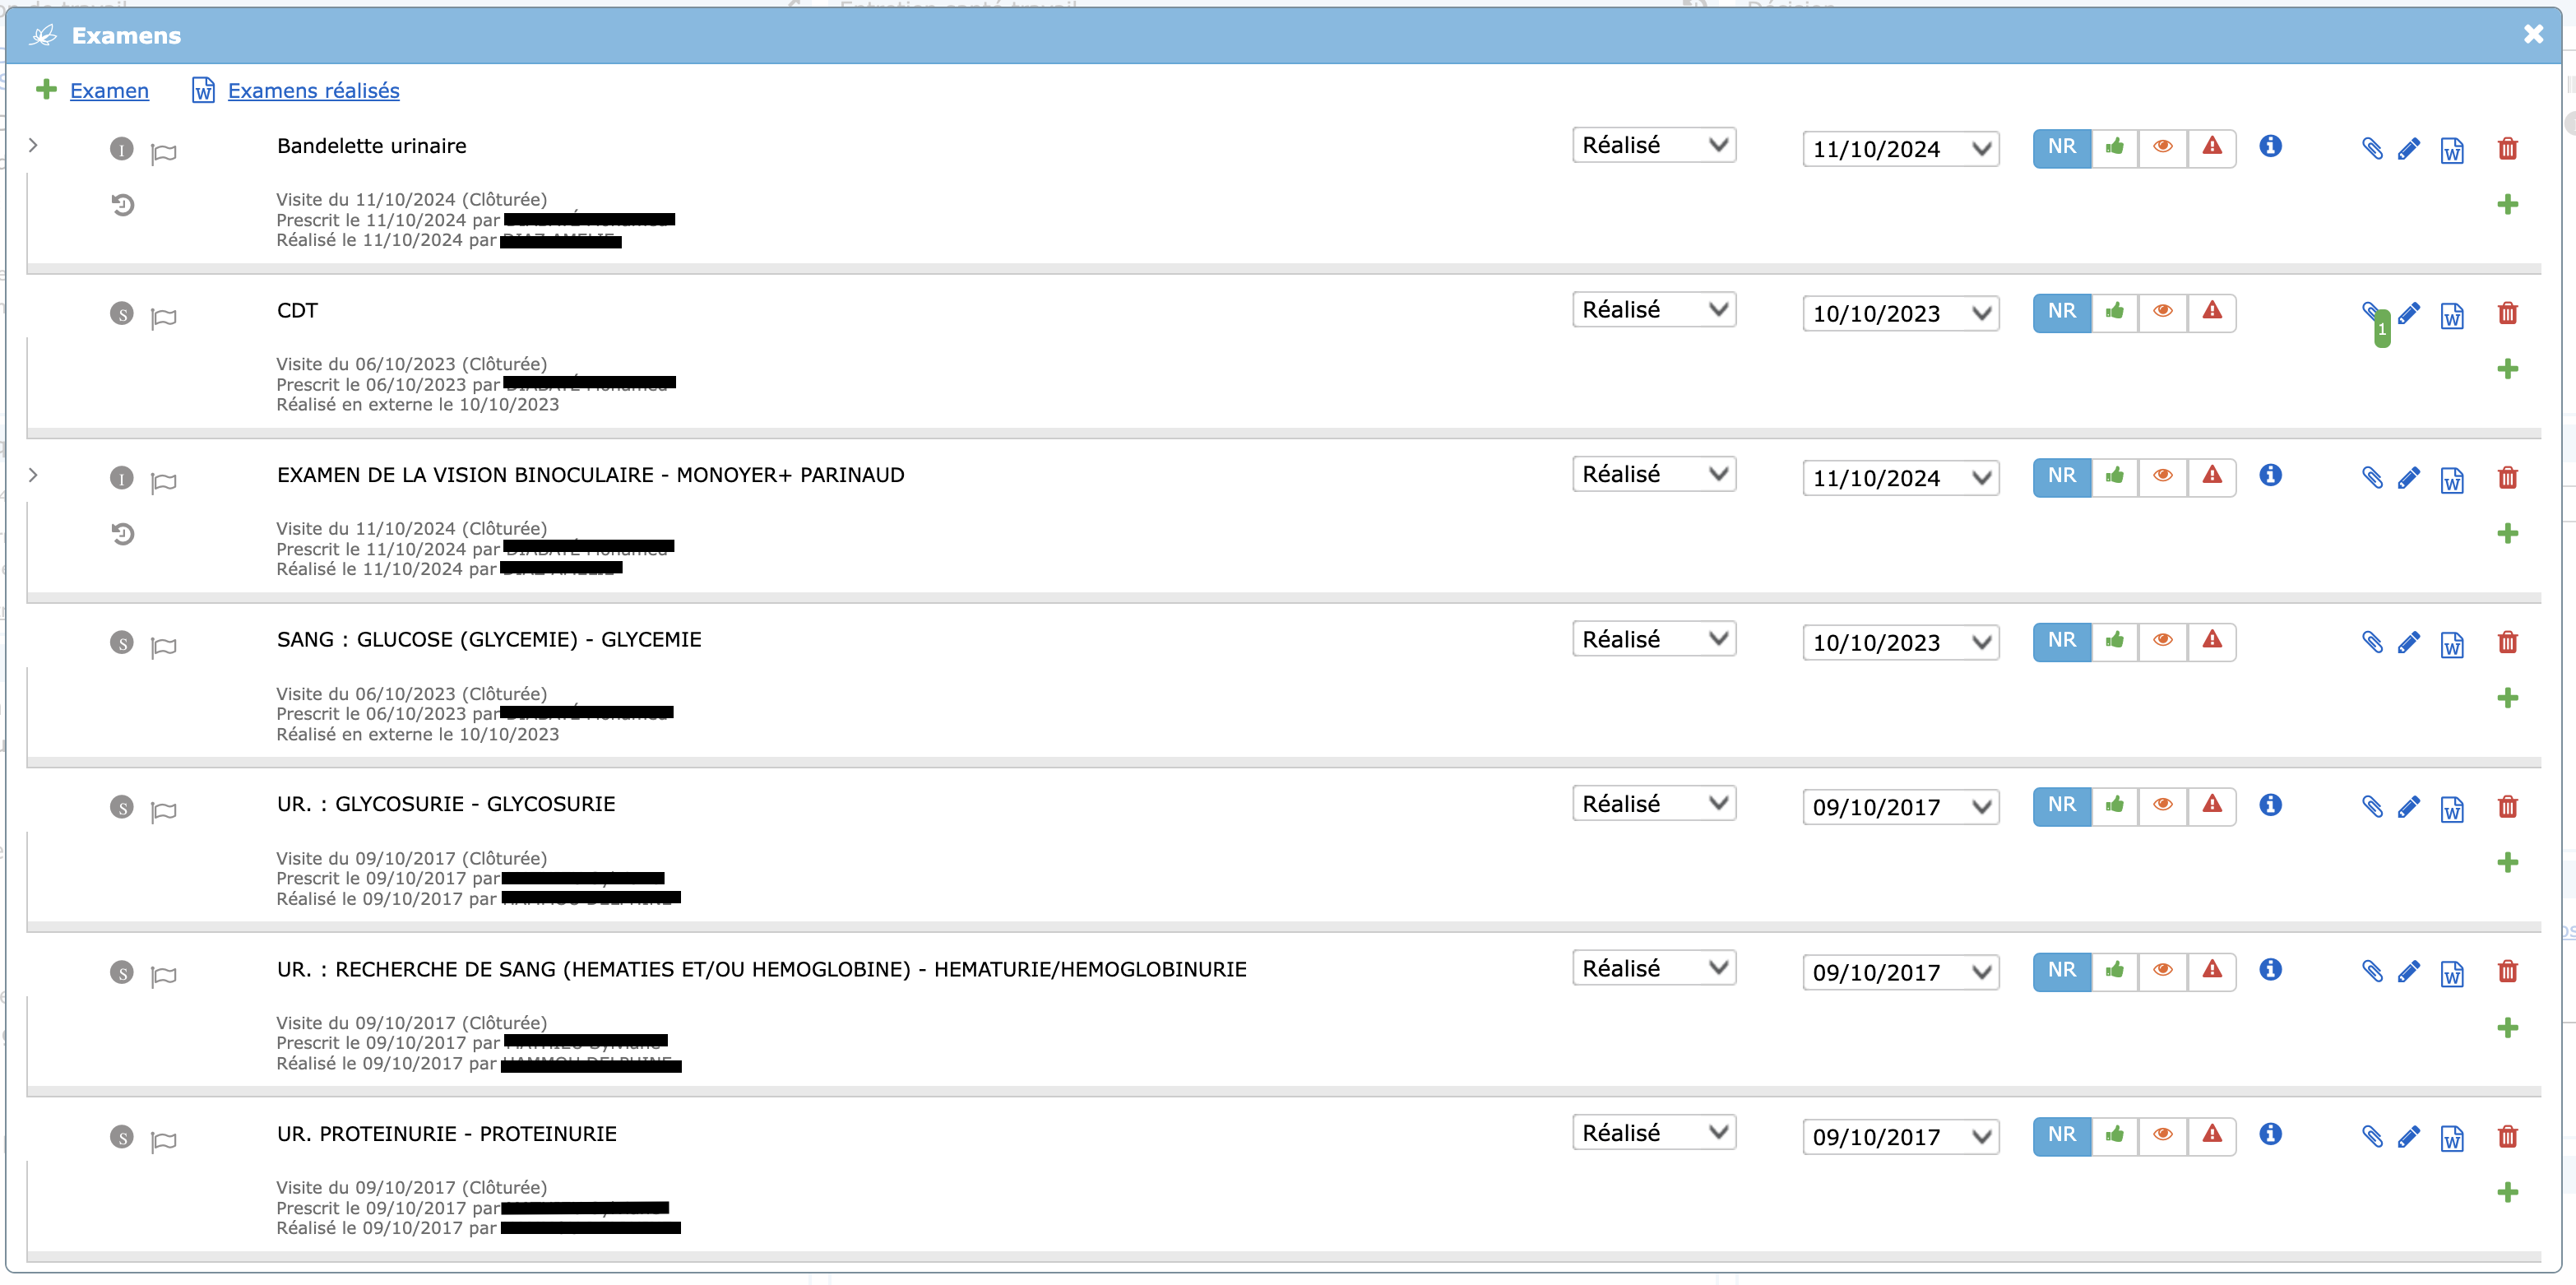
\includegraphics[width=\linewidth]{4_attachments/figures/preventiel_exam_full.png} % Remplacez "image2.png"
      \caption{Aperçu détaillé}
      \label{fig:image2}
  \end{subfigure}
  \caption{Examens sur préventiel}
  \label{fig:images}
\end{figure}
La localisation des données permet de valider avec le client les informations à extraire et de s’assurer que les ressources identifiées, comme les données relatives aux \textit{measure\_requests}, répondent bien aux besoins définis pour leur intégration dans le système Padoa.


\subsection{Exploration de la base de données du client}

L'étape qui suit consiste à explorer la base de données du client, qui constitue la source principale des informations à migrer. Cette phase implique une analyse détaillée de la structure et du contenu des données fournies via un dump. L'objectif est de comprendre l'organisation des tables, les relations entre elles, et les types de données stockées. 

Le client SSTI03 utilisait le logiciel préventiel avant de passer sur padoa, logiciel assez bien connu par l'équipe intégration car ce client n'est pas le premier à utiliser ce logiciel. La base de données de préventiel est donc assez connue de l'équipe et cette phase a donc été plutôt rapide.

Les informations nécessaires pour la migration des examens complémentaires en attente de résultat ont été identifiées (tables et liaisons) par rapport à ce qui avait déjà été fait.


\subsection{Requête pour les \textit{measure requests}}

Une fois l’exploration de la base de données du client terminée, la deuxième étape consiste à élaborer une requête spécifique dans l’outil Esquilo pour extraire les informations nécessaires liées aux \textit{measure\_requests}. 

La construction de la requête s’appuie sur les observations faites lors de l’analyse de la base. Il est important d’appliquer des filtres ou des conditions pour extraire uniquement les données nécessaires, tout en évitant les doublons ou les valeurs non conformes. Pour le cas des examens complémentaires en attente de résultat, on va se rendre compte qu'il suffit de récupérer les examens sans date de réalisation.

\begin{lstlisting}[language=SQL, caption=Aperçu de la requête]
  -- cte pour recuperer les employes actifs
  WITH flow_employees AS (
	{flow_employees}
)

SELECT element_dist.ID    AS measure_request_element_dist_source_id -- matricule examen
     , flow_employees.source_id   AS employee_source_id -- matricule employe
     , examen.DatePrescription    AS date_prescription -- requestedAt
     , consultation.ID    AS visit_histo_source_id -- numero visite
     -- beaucoup d'autres informations ...

FROM VIS_ElementDist element_dist
  INNER JOIN VIS_ExamenMedical examen   ON examen.IDElementDist = element_dist.ID
  INNER JOIN VIS_Dist dist    ON dist.ID = element_dist.IDDist
  -- Employee
  INNER JOIN  PersonnePhysique person   ON person.ID = dist.IDPersonnePhysique
  INNER JOIN flow_employees   ON flow_employees.ID = person.ID
  -- Jointures suppelementaires ... 

WHERE (examen.DateRetour IS NULL AND examen.DateRealisation IS NULL) -- i.e. en attente de resultat
  AND examen.DatePrescription IS NOT NULL
  AND examen.demande::integer <> 0 -- filtre les examens qui n'apparaissent a aucun endroit dans le front
;
\end{lstlisting}

Une difficulté majeure a été rencontrée à ce niveau car le client a demandé de reprendre une information qui n'était pas reprise avant: un statut particulier sur préventiel.
Cette information n'était pas reprise à la base dans la requête esquilo. Malheuresement pour nous, cette information visible sur l'ancien logiciel ne correspondait pas un champ d'une table de la base de donnée. Nous avons fini par comprendre après investigation que ce champ était calculé en fonction de certains autres champs de la manière suivante:

\begin{itemize}
  \item Refusé: si le champ refus est à 1
  \item Non demandé: Si le champ demande est à 0
  \item Prescrit: S'il y a une date de prescription
  \item Prévu: S'il y a une date de prévision
  \item Annulé: S'il y a une date d'annulation
\end{itemize}

Ces règles s'appliquent visiblement en cascade et sont exclusives.

\begin{lstlisting}[language=Python, caption=Calcul de statut]
  # Fonction pour calculer le champ
  def compute_status(row):
      if row['refus'] == 1:
          return 'Refuse'
      elif row['demande'] == 0:
          return 'Non demande'
      elif pd.notna(row['date_prescription']):
          return 'Prescrit'
      elif pd.notna(row['date_prevision']):
          return 'Prevu'
      elif pd.notna(row['date_annulation']):
          return 'Annule'
      return None

  ....
  # Application de la fonction
  df_measure_request['statut'] = df_measure_request.apply(compute_status, axis=1)
\end{lstlisting}

Une fois la requête rédigée et testée, elle est intégrée à l’esquilo pour automatiser l’extraction des \textit{measure\_requests}, en garantissant une récupération cohérente et exhaustive des données pour les étapes suivantes.


\subsection{Construction de l’extracteur et application des règles de transformation}

Une fois les requêtes SQL prêtes et exécutées via l’Esquilo, l’étape suivante consiste à construire un extracteur capable de traiter les fichiers CSV résultants. Cet extracteur a pour rôle de transformer les données brutes en appliquant les mappings de valeur validés avec le client, ainsi que les règles spécifiques à leur contexte. Le résultat est un \textit{dataframe} transformé, prêt pour les étapes suivantes de l’intégration.

Dans le cas spécifique du SSTI03, certaines règles métiers doivent être appliquées au contenu des \textit{measure\_requests}. Tout d’abord, seules les mesures ayant la mention \og prévu \fg{} ou \og prescrit \fg{} sont retenues pour la reprise. Ensuite, une règle supplémentaire impose que les mesures prescrites avant le \textbf{31 octobre 2022} se voient automatiquement cloturées donc ne seront pas reprises. Cette dernière règle aide le client à nettoyer ses données pour reprendre sur padoa avec une nouvelle base solide.

L’extracteur effectue ces traitements sur un dataframe pandas généré à partir du CSV d’entrée. Il commence par filtrer les lignes selon les critères établis (mentions \og prévu \fg{} ou \og prescrit \fg{}), puis applique les transformations nécessaires, comme la modification du statut pour les prescriptions antérieures à la date spécifiée. Une fois toutes les règles appliquées, un nouveau dataframe est produit, contenant uniquement les données conformes aux spécifications du client. Ce dataframe transformé est ensuite utilisé pour les étapes suivantes du pipeline d’intégration.

\subsection{Tests de l’extracteur avec \textit{pytest}}

Une étape essentielle dans le développement de l’extracteur consiste à tester son fonctionnement pour s’assurer qu’il produit des données conformes aux spécifications. Pour cela, la bibliothèque \textit{pytest} est utilisée, offrant un cadre puissant et flexible pour écrire et exécuter les tests unitaires.

Pytest est un framework de tests en Python très utilisé pour sa simplicité et sa flexibilité. Il permet de rédiger et d’exécuter des tests unitaires, fonctionnels ou d'intégration grâce à une syntaxe claire et concise\cite{wiki-pytest}. Pytest prend en charge des fonctionnalités avancées comme les tests paramétrés et des rapports détaillés. Ses fixtures permettent de configurer des environnements de test réutilisables, garantissant des conditions fiables pour chaque exécution. 

Les tests de l’extracteur reposent sur l’utilisation de données fictives, fournies sous forme de fichiers CSV simulant des cas réels. Ces fichiers incluent différents scénarios, comme des \textbf{measure\_requests} avec des statuts variés (\og prévu \fg{}, \og prescrit \fg{} ou autres) et des dates avant ou après le 31 octobre 2022. Le comportement attendu de l’extracteur est alors comparé aux résultats obtenus après transformation et nettoyage. Chaque test vérifie que les règles définies (filtrage des statuts, modification automatique du statut pour certaines dates, etc.) sont bien appliquées.

En parallèle, un test de \textbf{code coverage}\footnote{En génie logiciel, la couverture de code est une mesure utilisée pour décrire le taux de code source exécuté d'un programme quand une suite de tests est lancée\cite{wiki-coverage}} est automatiquement exécuté pour mesurer la couverture des tests sur le code écrit. Cet outil garantit que la majorité des fonctionnalités de l’extracteur sont vérifiées, réduisant ainsi le risque de bugs ou de comportements inattendus. Cette rigueur dans les tests permet d’assurer la fiabilité de l’extracteur avant son intégration dans le pipeline de reprise des données.
